\documentclass[xcolor=dvipsnames, 14pt]{beamer}
%\documentclass[xcolor=dvipsnames, bigger, aspectratio=169]{beamer}

\definecolor{AalborgBlue}{HTML}{211A52}
\usecolortheme[named=AalborgBlue]{structure}

\mode<presentation> {
	\usetheme[height=1.5em]{Rochester}
    %\usetheme{Frankfurt}
	\setbeamercovered{transparent}
}

\setbeamertemplate{navigation symbols}{}%remove navigation symbols
\setbeamertemplate{footline}[frame number]{}

\setbeamercolor{frametitle}{fg=white}
\setbeamercolor{title}{fg=white}
\setbeamercolor{navigation symbols dimmed}{fg=black!10}
\setbeamercolor{navigation symbols}{fg=black!30}
\setbeamercolor{section number projected}{fg=white}
\setbeamercolor{item projected}{fg=white}
\setbeamercolor{footlinecolor}{bg=AalborgBlue,fg=white} 


\usepackage[utf8x]{inputenc}
\usepackage[resetfonts]{cmap}
\usepackage{lmodern}
\usepackage[english]{babel}
\usepackage[T1]{fontenc}
\usepackage{graphicx}
\usepackage{microtype}
\usepackage{etoolbox}
\usepackage{multicol}
\usepackage{hyperref} % For hyperlinks in the PDF
\hypersetup{
    colorlinks=false,
    citecolor = red,
    urlcolor = blue
}

%\newcommand{\insertsectionandsubsection}[2]{%
%  \ifdefempty{#1}{}{
%    \ifdefempty{#2}{
%      #1
%    }{
%      #1: #2
%    }
%  }
%}

%\makeatother
%\setbeamertemplate{footline} %bottom frame
%{
%  \leavevmode%
%  \hbox{\begin{beamercolorbox}%[wd=\paperwidth,ht=2.5ex,dp=1.125ex,leftskip=.3cm,rightskip=.3cm plus1fil]{footlinecolor}%
%  \insertsectionandsubsection{\insertsection}{\insertsubsection}\hfill
%    \insertpagenumber/\inserttotalframenumber
%  \end{beamercolorbox}}%
%  \vskip0pt%
%}

\makeatletter
\AtBeginSection[]
{
  \begin{frame}<beamer>
    \frametitle{Next up}
    \small \tableofcontents[currentsection]
  \end{frame}
}

\newenvironment<>{blockyellow}[1]{%
  \setbeamercolor{block title}{fg=white,bg=yellow}%
  \begin{block}#2{#1}}{\end{block}}


\title[L2R Wikipedia Links]{Learning to Rank on Article Hyperlinks in Wikipedia}
\author{Blandine~Seznec \and Philip~Thruesen \and Jaroslav~Cechak \and Roel~Castano}
\institute{Aalborg University}
\date{\small June 28, 2016}

\begin{document}

\begin{frame}[noframenumbering, plain]
  \titlepage
\end{frame}

\begin{frame}
  \frametitle{Table of Contents}
  %\begin{columns}[t]
  %      \begin{column}{.5\textwidth}
  %          \footnotesize
  %          \tableofcontents[sections={1-5}]
  %      \end{column}
  %      \begin{column}{.5\textwidth}
  %          \footnotesize
  %          \tableofcontents[sections={6-10}]
  %      \end{column}
  %\end{columns}
  %\footnotesize
  %\begin{multicols}{2}    
  %  \tableofcontents[hideallsubsections]
  %\end{multicols}
  \small
  \tableofcontents
\end{frame}


% Roel - 1, 2, 3, 10
% Jaroslav - 8, 9
% Blandine - 6, 7
% Philip - 4, 5

% TITLE page: introduce people (and patrick thingy). Introduce title
% TOC page: Introduce what the presentation will be about

\section{Introduction and motivation}
\section{Introduction}

As technology becomes part of all aspects of human nature and new trends such as the internet of things connect everyday objects to the internet, the amount of data stored in the digital universe has been growing at an outstanding rate. Consequently, processing and analysing data sets has become increasingly difficult and techniques have been developed in the fields of machine learning, big data, and others to facilitate the use of data. \\
One of the many problems that arises from this growth of digital capacity is information retrieval. We can see examples of this with search engines, recommender systems, bioinformatics, and many more, where it is necessary to rank data sets based on relevance to a certain query taking into account multiple features which influence the relevance of each option. For cases like this ones, algorithms like Learning to Rank \\
One interesting case where Learning to Rank (L2R) could be applied is to extract the importance of links in Wikipedia articles to prevent Overlinking; Containing excessive number of links, making it difficult to likely to aid the user \cite{missing_links}. Wikipedia is an internet encyclopaedia with more than 38 million articles in over 250 different languages of semi-structured information. It is also the most popular wiki-based website, and is ranked by Alexa as the \#6 most popular website in the internet. It allows the collaborative modification of its articles by the users, which is one of the main reasons Wikipedia has grown to such an impressive size. \\
Being ``the free encyclopedia that anyone can edit'' has many advantages and disadvantages, and one of the disadvantages is, as mentioned before, Overlinking. As mentioned in a study by Ashwin Paranjape et al. \cite{paranjape}:  ``in the English Wikipedia, of all the 800,000 links added ... in February 2015, the majority (66\%) were not clicked even a single time in March 2015, and among the rest, most links were clicked only very rarely''. Since most of the editing of articles is done manually, finding and removing useless links to other articles is hard to do and editors do not focus on this. Given this case, we would like answer the following questions.

\begin{itemize}
\item Is it possible reduce the amount of links in Wikipedia articles by ranking the most relevant links based on a set of the most important features?
\item How could the features for the L2R algorithm be chosen for maximum effectiveness?
\item Will reducing the number of links in a Wikipedia article improve the readability of an article and aid the reader in finding interesting and relevant links?
\end{itemize}

% slide 1: wiki and overlinking
% slide 2: the figure 1 - converting to ranking problem
% slide 3: the 3 questions

\section{Steps of overall process}
% slide 4: procedure of how we worked. Visualized in a graph of some sort illustrating the work flow.
% steps to include: research datasets, define ranking problem, extract ground truth, construct features, feature selection and analysis, experimenting with L2R, evaluating results

\begin{frame}
  \frametitle{Overall Process}
  
  
  \begin{figure}[tbph]
    \centering
    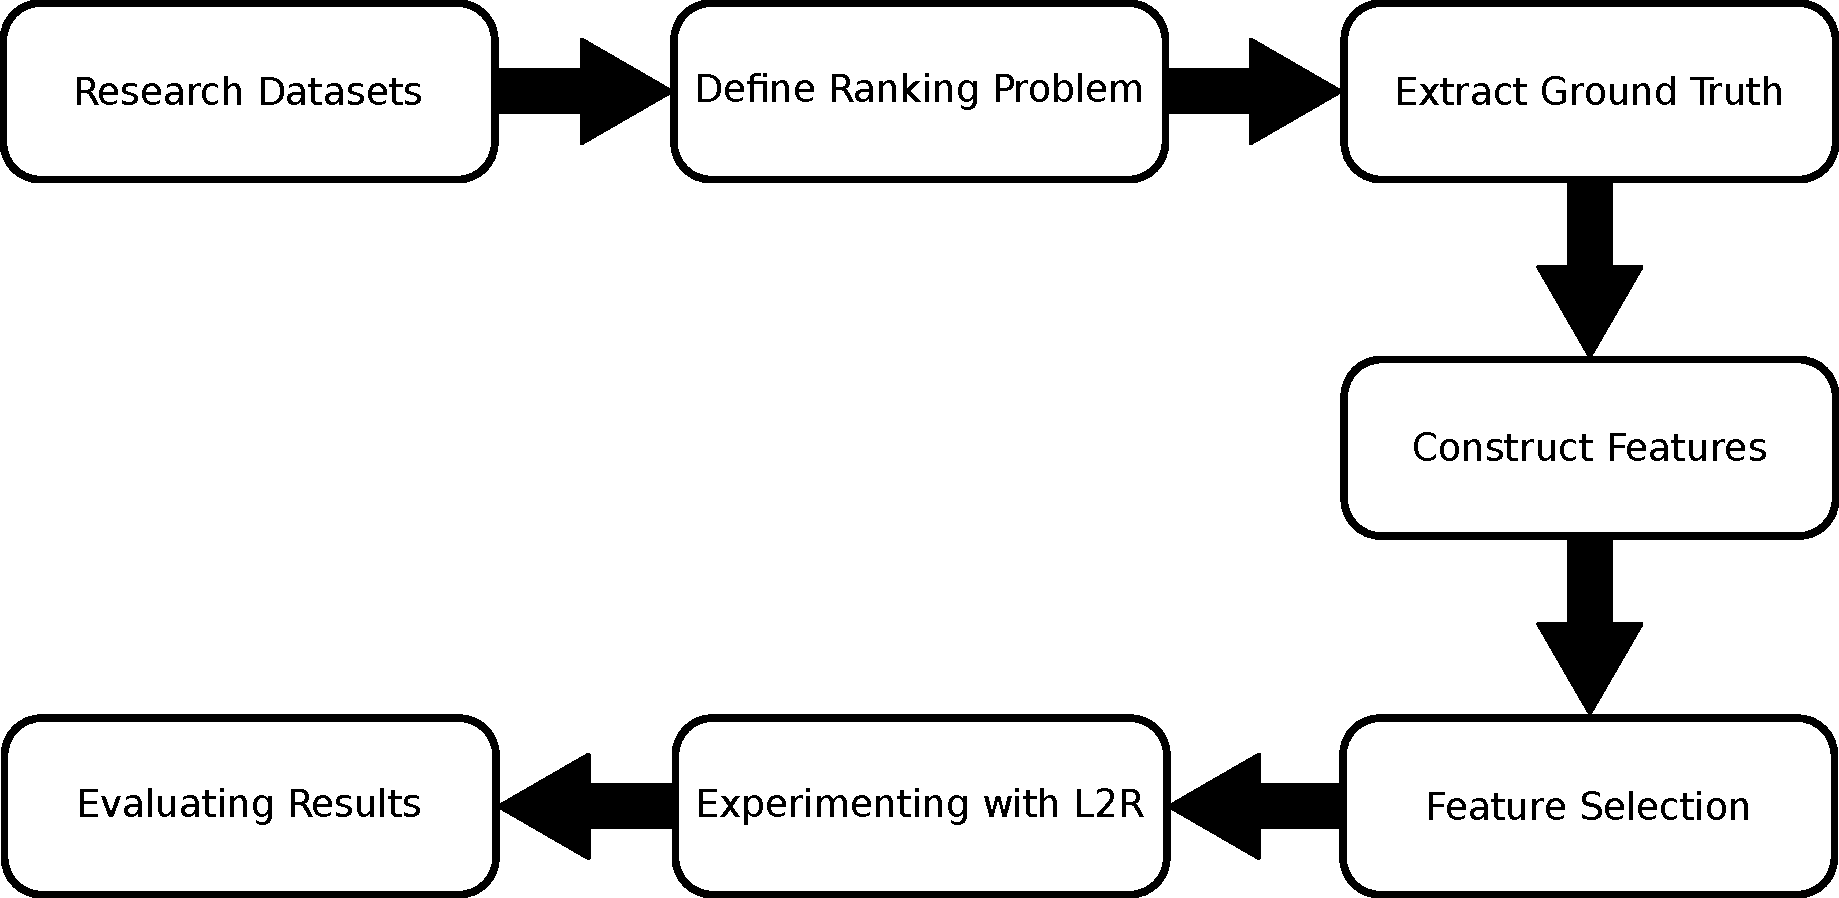
\includegraphics[width=\linewidth]{images/overall_process}
  \end{figure}
  
\end{frame}
% slide 4: procedure of how we worked. Visualized in a graph of some sort illustrating the work flow.
% steps to include: research datasets, define ranking problem, extract ground truth, construct features, feature selection and analysis, experimenting with L2R, evaluating results  

\section{Ranking}
% slide 5: explaining L2R method 
% slide 6: L2R approaches
% slide 7: RankLib

\begin{frame}
  \frametitle{Learning to Rank Method}
  
  \begin{figure}[tbph]
    \centering
    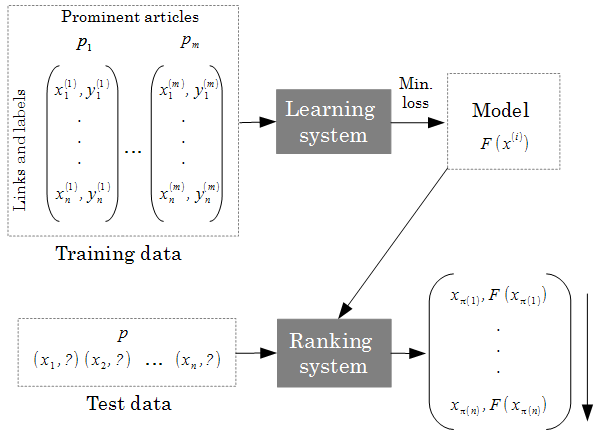
\includegraphics[width=\linewidth]{images/l2r}
  \end{figure}
  
\end{frame}

\begin{frame}
  \frametitle{L2R Approaches}
  \begin{block}{Pointwise}
   \begin{itemize}
    \item Each link is standalone instance.
    \item Input for Model: Feature Vector.
    \item Output for Model: Predicted Label.
    \item Loss Function: Based in single objects. Simplified to regression, classification, or ordinal regression.
  \end{itemize}
  \end{block}
\end{frame}

\begin{frame}
  \frametitle{L2R Approaches}
  \begin{block}{Pairwise}
   	\begin{itemize}
    	\item Considers pairs of links.
    	\item Input for Model: Pair of feature vectors.
    	\item Output for Model: Relative preference.
    	\item Loss Function: Discrepancy between preference predicted by the model and order in ground truth.
	  \end{itemize}
    \end{block}
\end{frame}

\begin{frame}
  \frametitle{L2R Approaches}
  \begin{block}{Listwise}
   	\begin{itemize}
    	\item Considers whole list of links.
    	\item Input for Model: List of feature vectors.
    	\item Output for Model: List of labels or permutation.
    	\item Loss Function: Directly measure final position/rank of links.
	  \end{itemize}
    \end{block}
\end{frame}

\begin{frame}
  \frametitle{RankLib}
  \centering
  	Library of Learning to Rank algorithms.
  \begin{figure}[tbph]
    \centering
    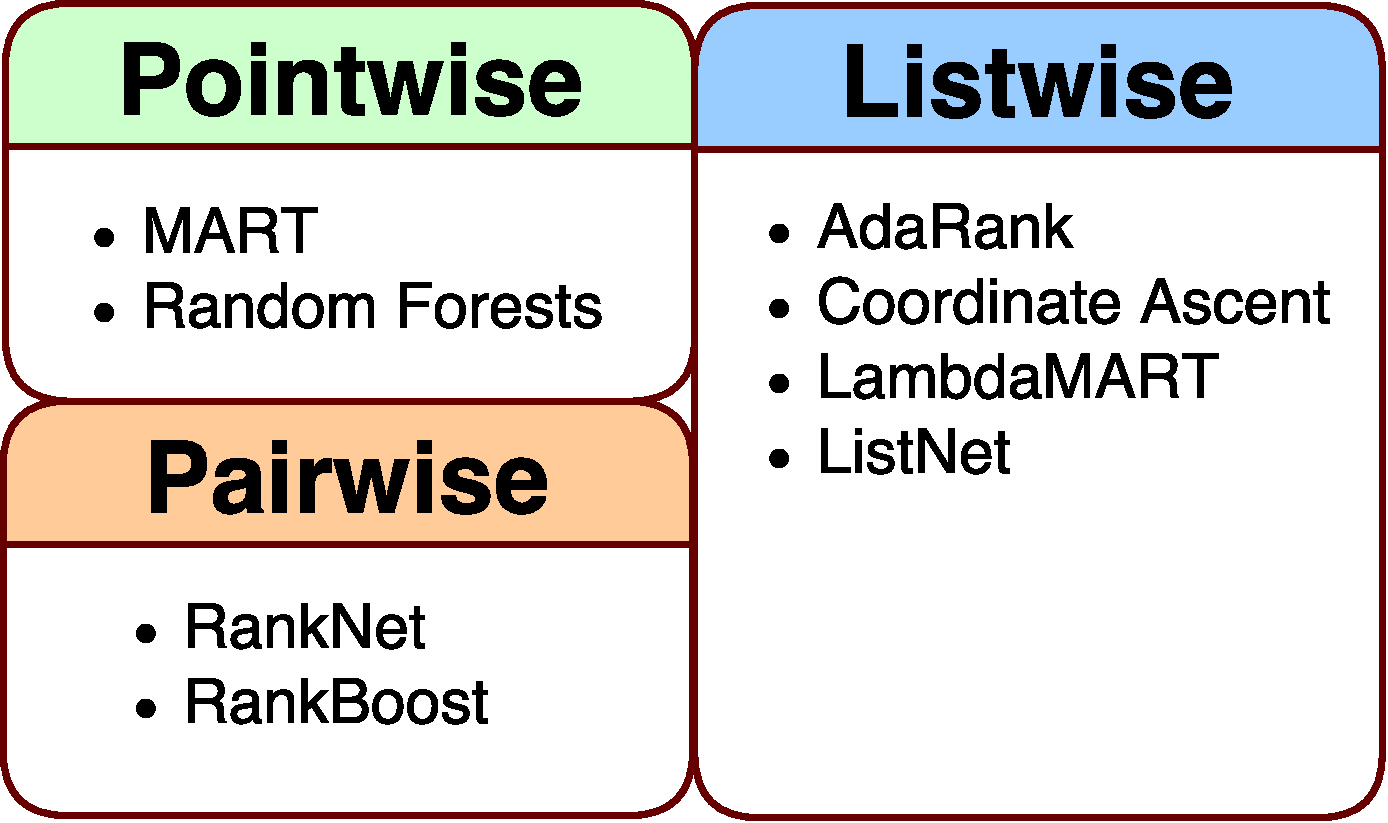
\includegraphics[width=0.7\linewidth]{images/RankLib}
  \end{figure}
\end{frame}



% slide 5: explaining L2R method 
% slide 6: L2R approaches
% slide 7: RankLib

\section{Datasets}
\subsection{Data Sets}

There are multiple data sets and sources available which facilitate the interaction with Wikipedia, and due to the massive amount of data managed by wikipedia, it is important to have an organised and manageable representation of this data in our own server for processing. This section describes the data sources used during the research of this article.

\subsubsection{Wikipedia Dumps}
The most significant data source is the English Wikipedia database dump, which is released at least once a month, and contains a complete copy of the text and metadata of current revisions of all articles in XML format. This dump facilitates the extraction of mu Wikipedia also releases the page views and page counts for all articles.

\subsubsection{Wikipedia Clickstream}
The Wikipedia Clickstream \cite{wulczyn} project contains data sets of $(referer, resource)$ pairs of articles describing user navigation and raw counts on the volume of traffic through the article pairs. This pairs are extracted from the request logs of Wikipedia, in which the referer is an HTTP header field that identifies the webpage from which the resource was requested. Typical referral sites like Google or Facebook are also included and crawler-traffic has been attempted filtered from the raw data.
% slide 8: overview listing datasets we used
% slide 9: Wiki dumps
% slide 10: wiki clickstream

\section{Ground truth and training data}
\subsection{Ground Truth}
\label{sec:groundtruth}

James Kobielus \cite{kobielus}, from IBM Big Data and Analytics Hub, describes ground truth as ``a golden standard to which the learning algorithm needs to adapt''. In most cases, a training dataset labeled by human experts is needed to provide data patterns for the learning algorithm to use as baseline. This type of machine learning is referred to as supervised learning. The other two main approaches, unsupervised learning and reinforcement learning, aim to automate this process from the data itself, not labeled by humans.

In our case we apply a supervised learning model using a ground truth dataset constructed primarily from the clickstream data query logs. We use a subset of 1000 articles having the most outgoing clicks. We refer to these articles as being the \textit{prominent} articles. Each of these prominent articles contain links to other articles which add to a total of 144k uniquely referenced articles and 283k article $(p,\beta)$ pairs where $p$ is a prominent article and $\beta$ is a \textit{prominent-linked} article.

%feature table has to be here so that it can be displayed on the next page
\newcolumntype{M}[1]{>{\raggedright}m{#1}}
\begin{table*}[t!]
\caption{Summary of all features used for L2R algorithm}
\centering
\label{features_tab}
\begin{tabular}{lM{0.5\textwidth}l}

\centering
\textbf{Feature name} & \textbf{Description} & \textbf{Section} \\
\toprule
Popularity of resource & Processed measure on article views coming from external search engines and social media. & \ref{popularity of resource}\\
\midrule
Popularity percentile rank & Measure extracted from local distributions of article views coming from external search engines and social media. & \ref{popularity percentile rank}\\
\midrule
Link position & Position of the link deduced from its distance to the beginning of the article. & \ref{link position}\\
\midrule
Link order & Relative position in the article according to the order of appearances of all links. & \ref{link order}\\
\midrule
Link count & Number of occurrences of the link in the article. & \ref{link count}\\
\midrule
Community membership & Binary value detecting if two articles belong to the same "community" (i.e. to the same cluster of articles). & \ref{community membership}\\
\midrule
Symmetric linking & Binary value detecting if two articles both link one to each other. & \ref{symmetric linking}\\
\midrule
Hits and PageRank & Score based on the number of edges in the graph representation and on the neighbours score. Give an idea of how general the article topic is. & 
\ref{hits and pagerank}\\ 
\midrule
Relatedness & Relatedness of two articles computed on the number of links (both outgoing and incoming links) they have in common. & \ref{relatedness obtained from links}\\
\midrule
Textual similarity & Semantic comparison between two article text content implemented using cosine similarity on TF-IDF vectors. & \ref{textual similarity}\\
\midrule
Title similarity & Similarity between two article titles implemented using Jaccard coefficient on the title words. & \ref{title similarity} \\
\bottomrule
\end{tabular}
\end{table*}

The clickstream data does not contain pairs where the number of referrals from $p$ to $\beta$ is below 10 and therefore we supplement our ground truth data using the Wikipedia article dumps for the same period of time as the recording of clickstream data. In this way, we can extract article pairs that do not appear in the clickstream data because of the 10-click limit (set to protect privacy) -- this adds a substantial amount of ``unpopular'' article links to our set so that we avoid a bias towards more clicked links.
% slide 11: introducing ground truth
% slide 12: selection and extraction of prominent articles
% slide 13: constructing ground truth file w. figure 3
% slide 14: constructing rankLib file
% slide 14.5: table 6, experimental setup for supervised learning
% slide 14.7: difficulties and solutions for working with the wikipedia data

\section{Features}
% slide 15: overview of features. Include list of feature names and highlight ones to describe in detail next.
\begin{frame}
  \frametitle{Features}
    \begin{itemize}
     \item Link properties
      \begin{itemize}
       \item position
       \item order
       \item count
       \item symmetric linking
      \end{itemize}
      
      \item Popularity 
      \begin{itemize}
       \item popularity of resource 
       \item popularity of percentile rank
      \end{itemize}
      
      \item Articles similarity
      \begin{itemize}
       \item link relatedness
       \item text similarity
       \item title similarity
      \end{itemize}

   \item Community membership
   \item Hits and PageRank

  \end{itemize}
\end{frame}


% slide 16: simple link feature introduction: link order
\begin{frame}
  \frametitle{Link order}
      \begin{figure}[h]
   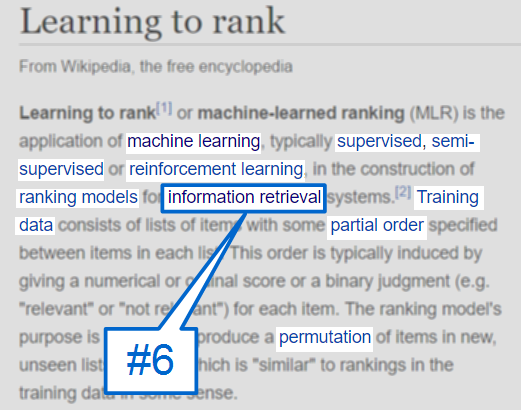
\includegraphics[height=0.6\textheight]{images/link_order}
  \end{figure}
  \begin{itemize}
    \item Motivation:
    \begin{itemize}
     \item Readers habit to read first paragraphs
     \item Main concepts in the leading section
	\end{itemize}
    \item Extracted from Wikipedia dumps
  \end{itemize}
\end{frame}

% slide 17: link symmetry
\begin{frame}
  \frametitle{Symmetrical linking}
  
  \begin{figure}[h]
   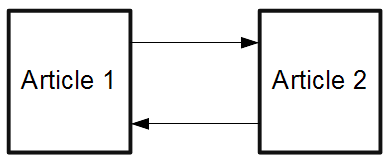
\includegraphics[width=0.75\textwidth]{images/symmetry}
  \end{figure}
  
   \begin{itemize}
   \item Binary feature
   \item Motivation: Highly related topics 
   \item Extracted from Wikipedia dumps
   \end{itemize}

\end{frame}

% slide 18: Motivaltion for similarity features
% slide 19: "Text similarity" feature
\begin{frame}
  \frametitle{Similarity features}
  Measuring relatedness of two linked articles  
\begin{itemize}
\item Text
\item Links
\item Title
\end{itemize}
\textbf{Motivation}: users are more likely to switch to a related topic  
\end{frame}

\begin{frame}
  \frametitle{Example: "Text similarity"}
  \begin{itemize}
\item Measure semantic similarity between two articles 
\item Extract text from Wikipedia dumps
\end{itemize}

    \begin{figure}[h]
    \centering
   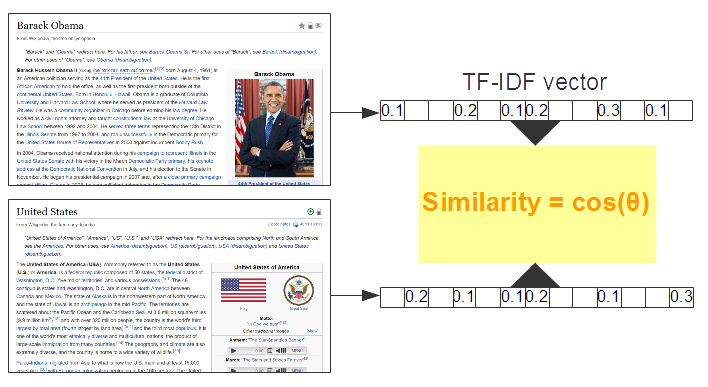
\includegraphics[height=0.75\textheight]{images/similarity}
  \end{figure}
\end{frame}

% slide 20: Motivation for community features
% slide 21: "Community 3" feature
\begin{frame}
   \frametitle{Community features}
\begin{itemize}
\item Graph representation
\item \textbf{Communities}: clusters of interconnected articles
\end{itemize}
\textbf{Motivation}: Two articles of the same community should discuss a similar topic

  \begin{figure}[h]
   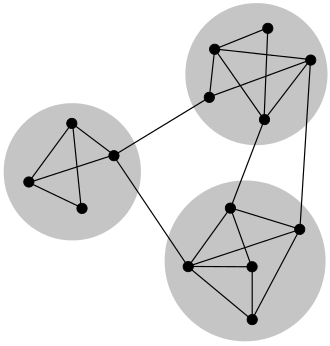
\includegraphics[height=0.4\textheight]{images/communities}
   \caption{Sketch of a small network displaying community structure}
  \end{figure}
 
\end{frame}

\begin{frame}
   \frametitle{Example: "Community 3"}
   \begin{itemize}
\item Extract links from Wikipedia dumps
\item Build the graph
\begin{itemize}
\item Vertices: articles
\item Edges: links
\end{itemize}
\item Distinguish communities with InfoMAP algorithm
\end{itemize}
Binary feature: 1 if both articles belongs to the same community, 0 otherwise
\end{frame}

% slide 22: Motivation for Interest features
% slide 23: "Search Interest" feature
\begin{frame}
   \frametitle{Interest features}
   \textbf{Interest}: number of page views

   \begin{itemize} 
   \item Extracted from Clickstream data
   
   \begin{itemize}
\item External traffic from Google, Yahoo and Bing
\item External traffic from Facebook and Twitter

\end{itemize}
\item Does not depend on current article
\end{itemize}
   \textbf{Motivation}: Readers may have a tendency to follow links to articles on trending and popular topics.
   
\end{frame}

\begin{frame}
   \frametitle{Example: "Search Interest"}
     \begin{figure}[h]
   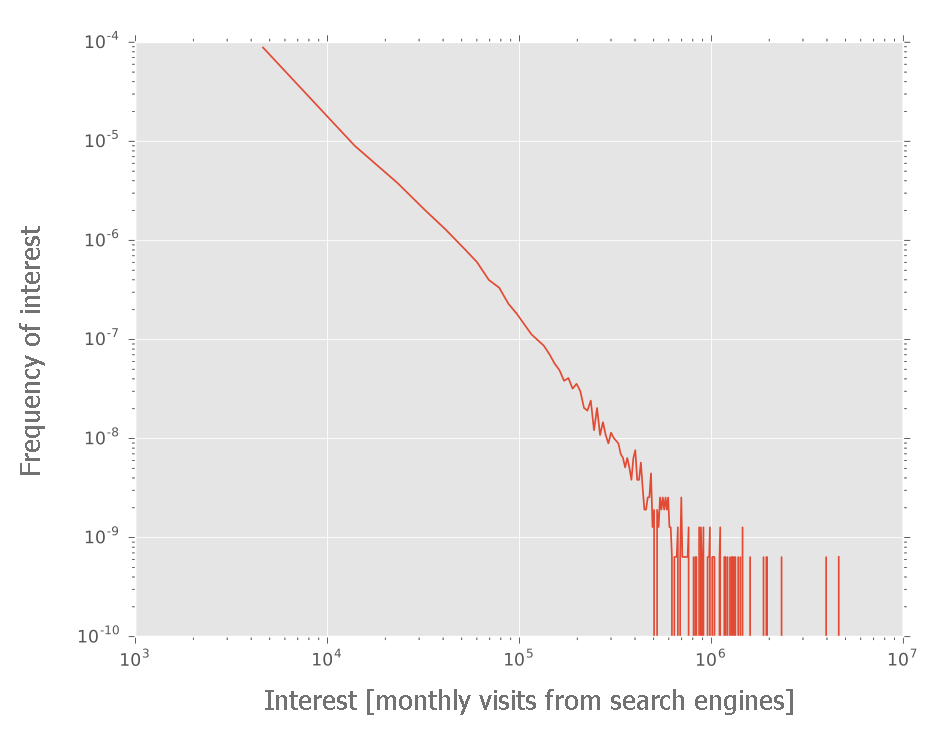
\includegraphics[height=0.6\textheight]{images/pwl_graph}
  \end{figure}
   
   \begin{itemize}
\item Search traffic assumed driven by social networks
\item Social networks form scale-free graphs
\item Interest follows a power law distribution
\item Feature defined by logarithm of search interest
\end{itemize}
   
\end{frame}
% slide 15: overview of features. Include list of feature names and highlight ones to describe in detail next.

% slide 16: simple link feature introduction: link order
% slide 17: link symmetry

% slide 18: Motivaltion for similarity features
% slide 19: "Text similarity" feature

% slide 20: Motivation for community features
% slide 21: "Community 3" feature

% slide 22: Motivation for Interest features
% slide 23: "Search Interest" feature

\section{Feature analysis}
% slide 24: introduce 3 methods and formula for finding importance of feature and how some were filtered because of redundance.

\begin{frame}
\frametitle{Feature Analysis}
Importance of a feature: 3 metrics
\begin{itemize}
\item \textbf{Info Gain}:
{\small $ InfoGain(Rank,Feature) = H(Rank) - H(Rank | Feature) $}
\item \textbf{PCA} (Principal Component Analysis): projection onto a single dimension
\item \textbf{CFS} (Correlation Feature Selection): subsets with low inter-correlation and high correlation with rank
\end{itemize}
\end{frame}

\begin{frame}
\frametitle{Feature Selection}
\begin{itemize}
\item \textbf{"Top 6"} (using Usefulness metric):
$$u_{f_i} = \frac{infogain_{f_i}}{\max(infogain_{f_j})} + \frac{|pca_{f_i}|}{\max(|pca_{f_j}|)} + \frac{cfs_{f_i}}{\max(cfs_{f_j})}$$

\item \textbf{"Non zero Info Gain"}
\end{itemize}



\end{frame}
% slide 24: introduce 3 methods and formula for finding importance of feature and how some were filtered because of redundance.

\section{Evaluation methods}
% slide 25: introduction and overview of 3 methods
% slide 26: NDCG method ("industry standard") 
% slide 27: The 191 method
% slide 28: Improved method

\begin{frame}
  \frametitle{Used evaluation metrics}
  \begin{enumerate}
    \item normalized discounted cumulative gain (NDCG)
    \item precision (P)
    \item query sensitive precision (PP)
    \item $@k$ suffix
  \end{enumerate}
\end{frame}

\begin{frame}
  \frametitle{Normalized Discounted Cumulative Gain}
  \begin{itemize}
    \item gain
    \item cumulative
    \item discounted
    \item normalized    
  \end{itemize}
  \begin{exampleblock}{Example}
    \begin{description}
      \item[links] $l_1$, $l_2$, $l_3$, $l_4$, $l_5$
      \item[labels] $y_1=5$, $y_2=4$, $y_3=3$, $y_4=2$, $y_5=1$\\
      \item[ranking] $l_1$, $l_5$, $l_3$, $l_4$, $l_2$
      \item[NDCG@3] $\frac{1}{30.074} (\frac{2^5-1}{log_2(3)} + \frac{2^1-1}{log_2(4)} + \frac{2^3-1}{log_2(5)}) = 0.7672$
    \end{description}
  \end{exampleblock}
\end{frame}

\begin{frame}
  \frametitle{Precision}
  \begin{itemize}
    \item a generalised version for binary labels
    \item better or equal to the label at the position $k$
    \item number of links per query vary
  \end{itemize}
  \begin{exampleblock}{Example}
    
    \begin{description}
      \item[links] $l_1$, $l_2$, $l_3$, $l_4$, $l_5$
      \item[labels] $y_1=5$, $y_2=4$, $y_3=3$, $y_4=2$, $y_5=1$\\
      \item[ranking] $l_1$, $l_5$, $l_3$, $l_4$, $l_2$
      \item[P@3] $\frac{1}{3} (1 + 0 + 1) = 0.6667$
    \end{description}
  \end{exampleblock}
\end{frame}

\begin{frame}
  \frametitle{Limitations of precision}
  \begin{figure}[tbph]
    \centering
    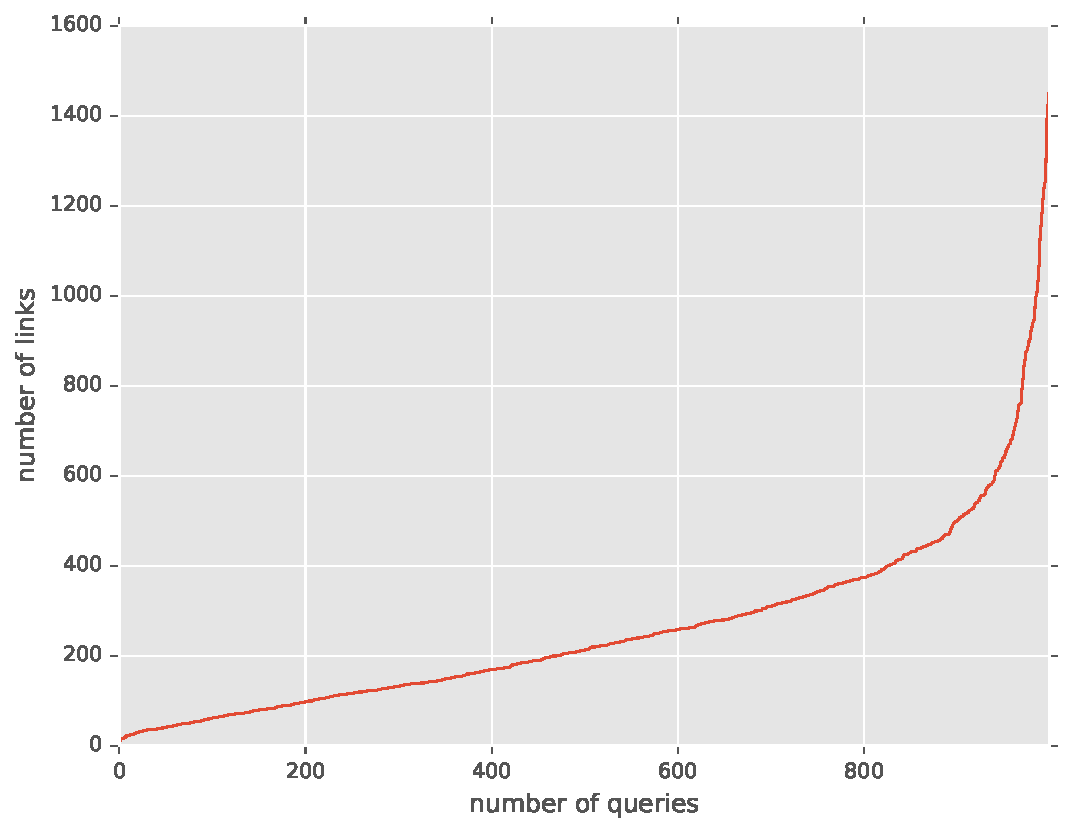
\includegraphics[width=0.95\linewidth]{images/limits_of_precision}
  \end{figure}
\end{frame}

\begin{frame}
  \frametitle{Query sensitive precision}
  \begin{itemize}
    \item different number of links per query
    \item a precision with the relative position in percentage
  \end{itemize}
  \begin{exampleblock}{Example}
    \begin{description}
      \item[links] $l_1$, $l_2$, $l_3$, $l_4$, $l_5$
      \item[labels] $y_1=5$, $y_2=4$, $y_3=3$, $y_4=2$, $y_5=1$\\
      \item[ranking] $l_1$, $l_5$, $l_3$, $l_4$, $l_2$
      \item[PP@50] $\frac{1}{3} (1 + 0 + 1) = 0.6667$
    \end{description}
  \end{exampleblock}
\end{frame}

\begin{frame}
  \frametitle{Limitations of query sensitive precision}
  \begin{figure}[tbph]
    \centering
    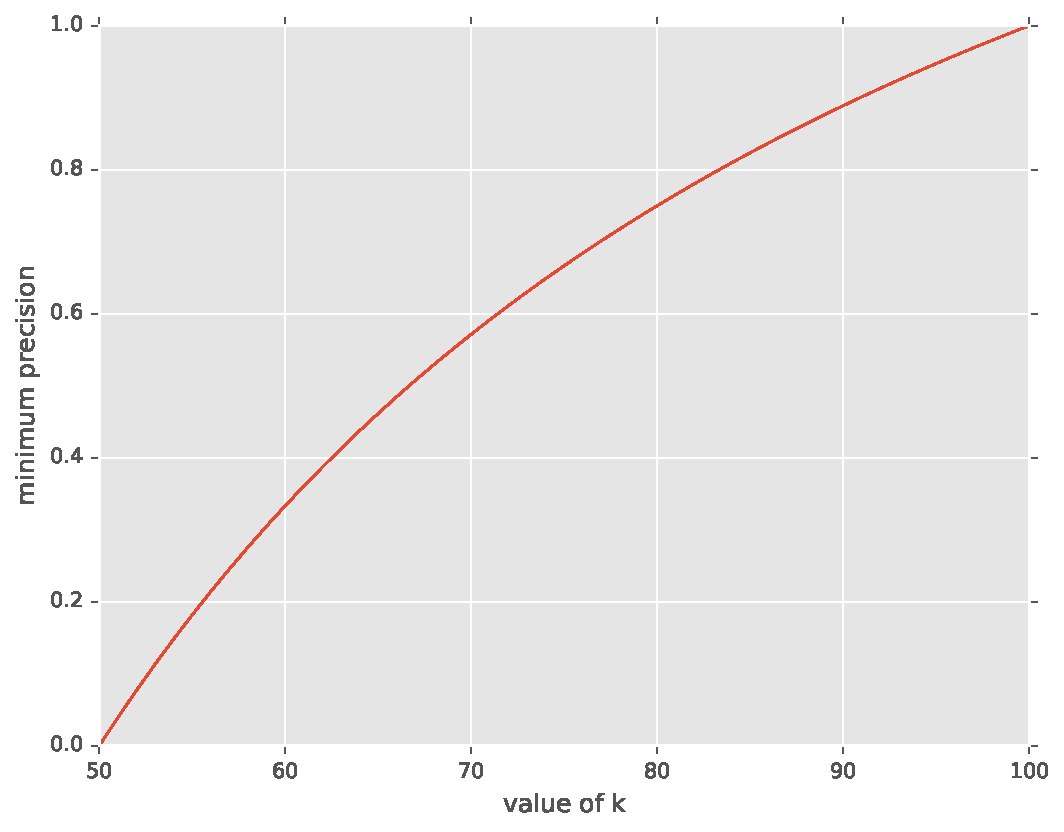
\includegraphics[width=0.95\linewidth]{images/limits_of_percentage_precision_new}
  \end{figure}
\end{frame}
% slide 25: introduction and overview of 3 methods
% slide 26: NDCG method ("industry standard") 
% slide 27: The 191 method
% slide 28: Improved method

\section{Results}
% slide 29: visualize results in bar chart. Select important algos and have 4 bars (each of eval. methods)
% slide xx: some more slides with e.g. zeros..
% slide xx: examples of ranking

\begin{frame}
  \frametitle{Results for NDCG@10}
  \begin{figure}[tbph]
    \centering
    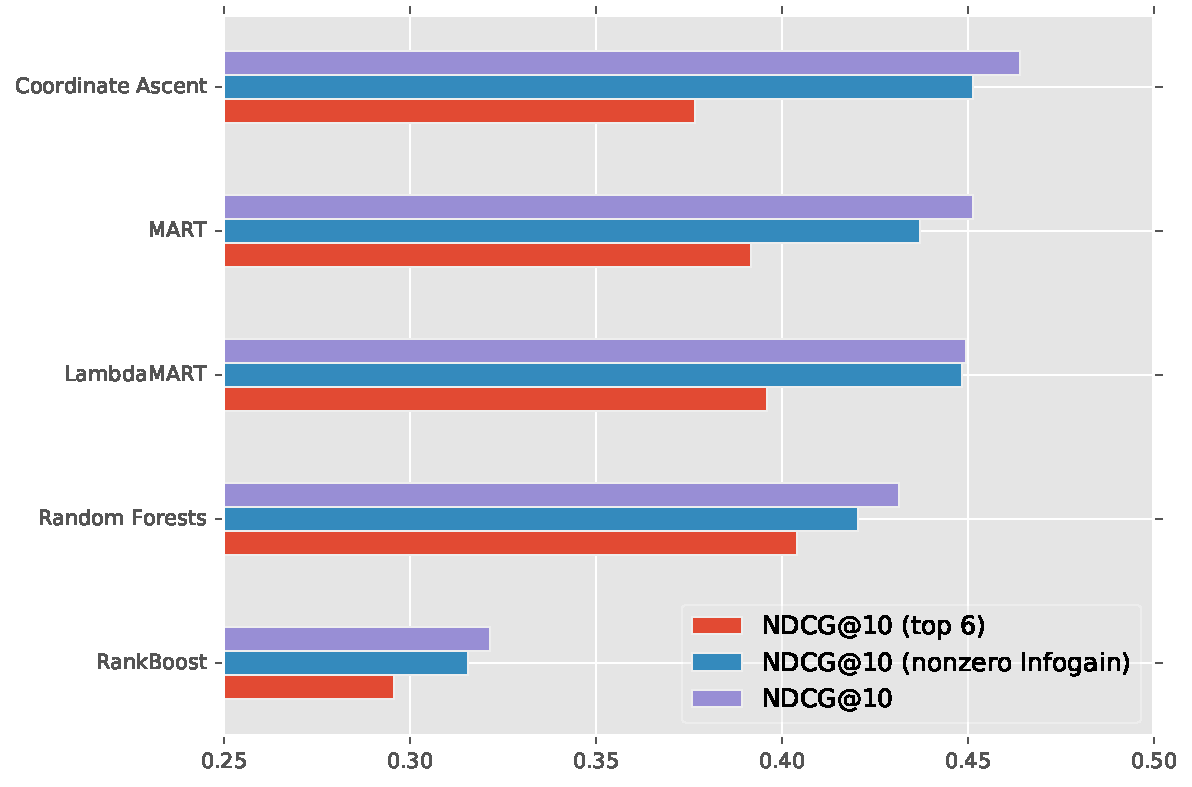
\includegraphics[width=\linewidth]{images/results_ndcg10}
  \end{figure}
\end{frame}

\begin{frame}
  \frametitle{Results for P@191}
  \begin{figure}[tbph]
    \centering
    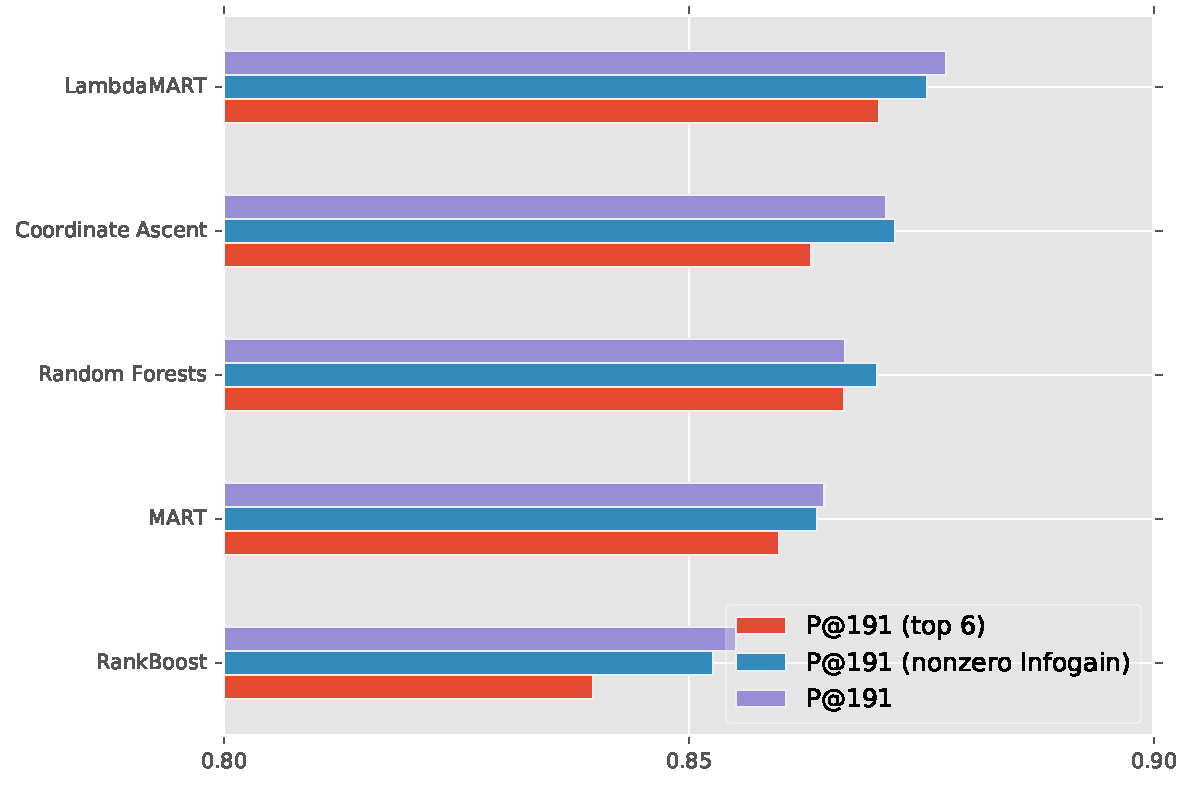
\includegraphics[width=\linewidth]{images/results_p191}
  \end{figure}
\end{frame}

\begin{frame}
  \frametitle{Results for PP@75}
  \begin{figure}[tbph]
    \centering
    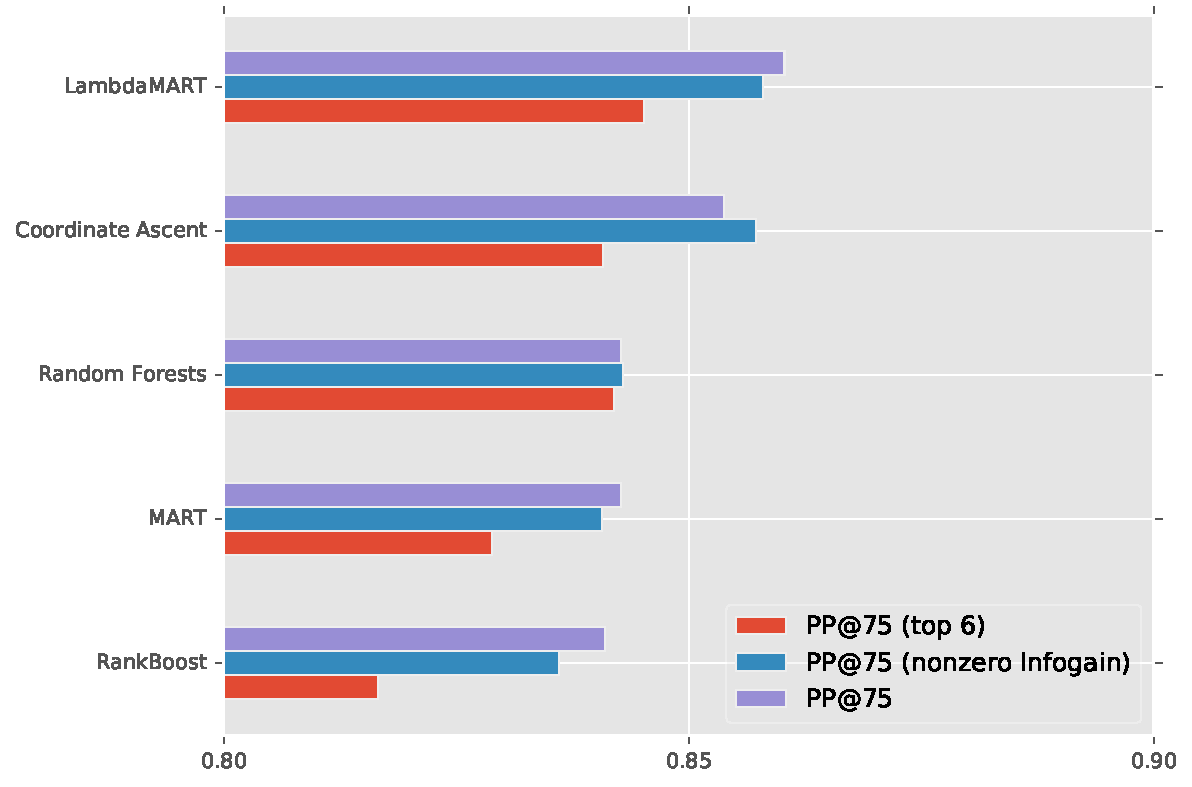
\includegraphics[width=\linewidth]{images/results_pp75}
  \end{figure}
\end{frame}

\begin{frame}
  \frametitle{Results for PP@50}
  \begin{figure}[tbph]
    \centering
    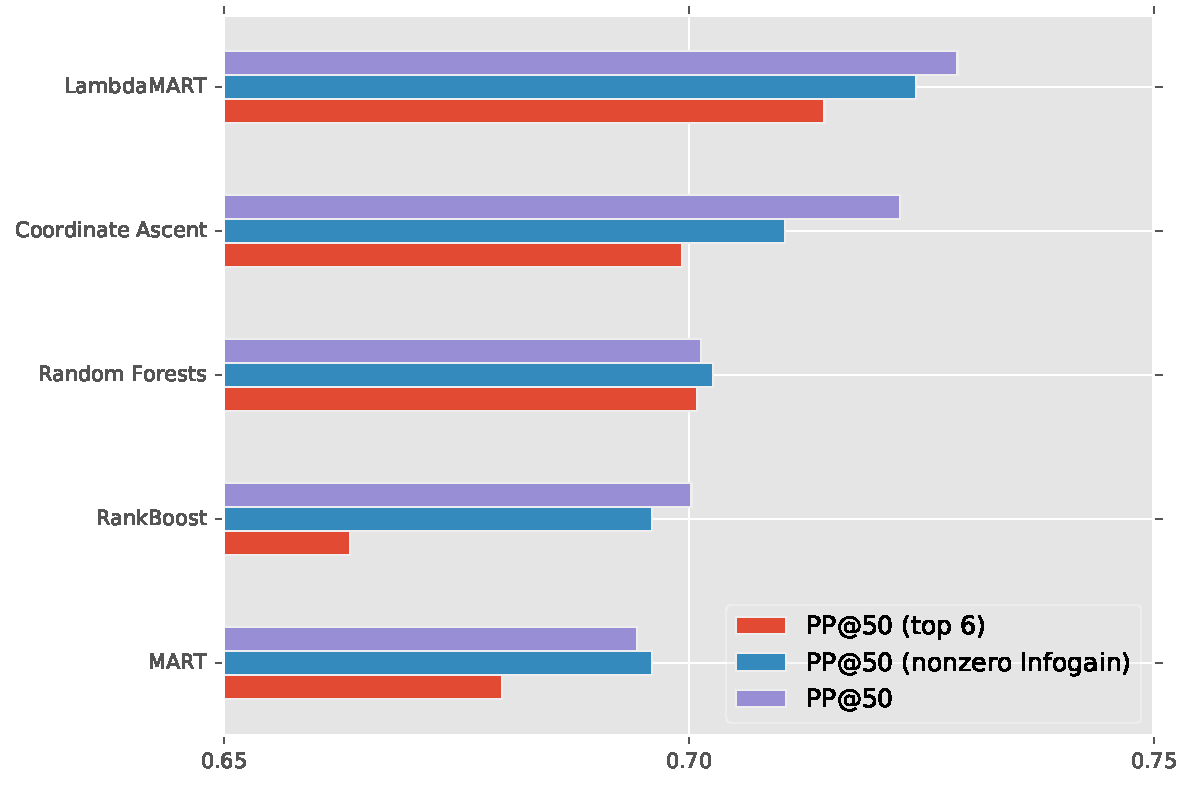
\includegraphics[width=\linewidth]{images/results_pp50}
  \end{figure}
\end{frame}

\begin{frame}
  \frametitle{Results for PP@k for various k}
  \begin{figure}[tbph]
    \centering
    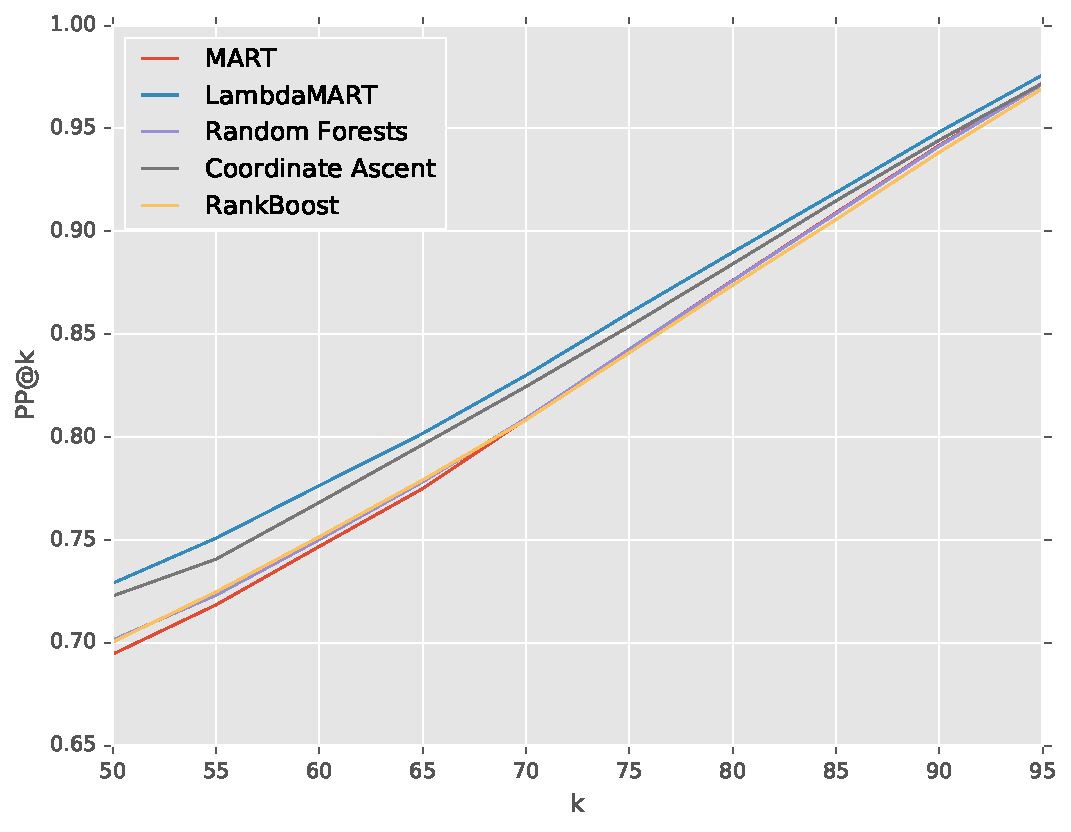
\includegraphics[width=0.95\linewidth]{images/results_pp_k}
  \end{figure}
\end{frame}

\begin{frame}
  \frametitle{Comparison of learning times}
  \begin{figure}[tbph]
    \centering
    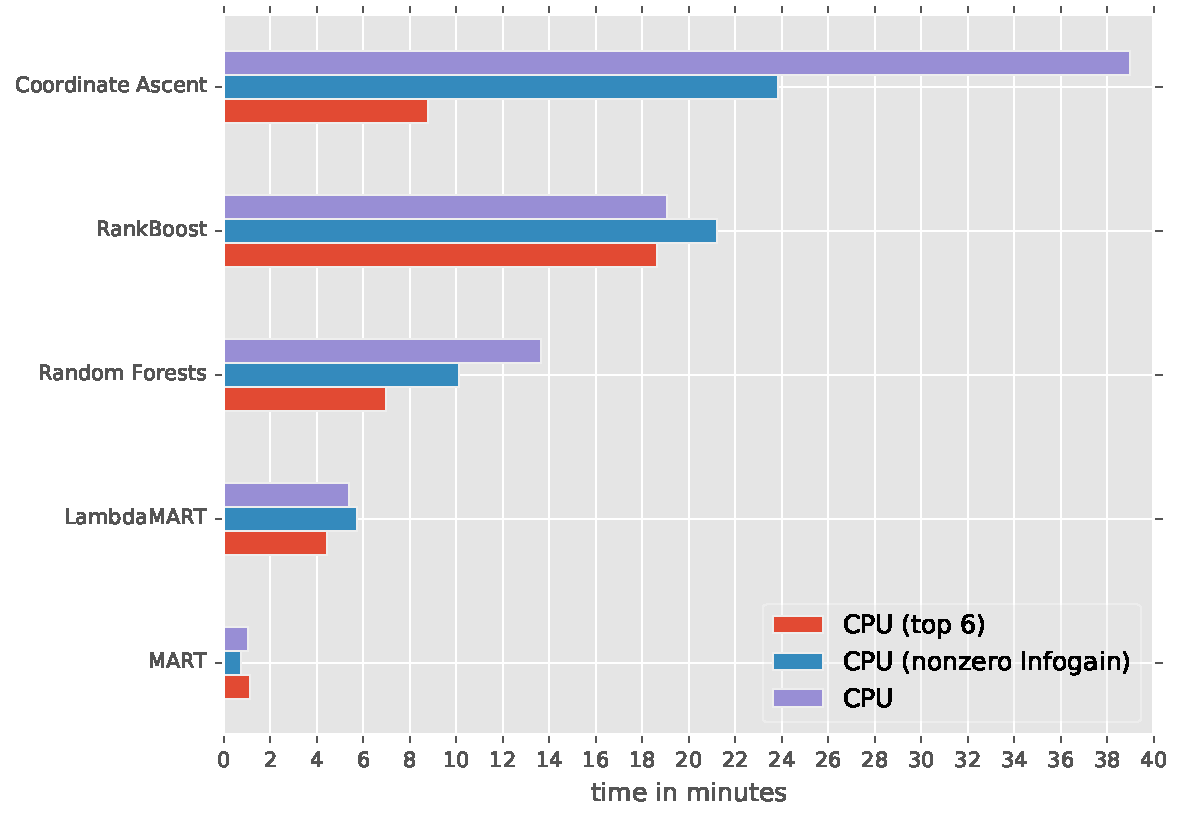
\includegraphics[width=0.95\linewidth]{images/results_times}
  \end{figure}
\end{frame}
% slide 29: visualize results in bar chart. Select important algos and have 4 bars (each of eval. methods)
% slide xx: some more slides with e.g. zeros..
% slide xx: examples of ranking

\section{Discussion and conclusion}
\section{Discussion}

\paragraph{Feature Selection}
Reasons for feature selection are to reduce overfitting and eliminate possible truly redundant features -- moreover, reducing the number of features can simplify the model and make it easier to interpret. In this work we focused mainly on potential performance benefits, but the results from table \ref{tab:feature_relevance} can also be useful for identifying feature subsets with potential to outperform full set. For example, taking only features with non-zero Infogain is one possible approach.
% * <philip@thruesen.dk> 2016-06-01T19:00:00.702Z:
%
% outcommented a paragraph. I dont believe using a subset of features will ever perform better than the full set unless there's overfitting which I think is very unlikely for our model.
%
% ^ <jarekcechak@gmail.com> 2016-06-02T09:10:39.850Z:
%
% This is what Nattiya told us that feature selection is usually used for
%
% ^ <jarekcechak@gmail.com> 2016-06-02T09:10:44.022Z.
% * <philip@thruesen.dk> 2016-06-01T18:56:01.192Z:
%
% > truly redundant
%
% changed conflicting to truly redundant. Change back if you disagree
%
% ^ <roelcastanomoreno@gmail.com> 2016-06-02T09:12:22.872Z.

All three methods used to evaluate the features are only heuristics and don't completely reflect true value of features. They are mainly focused on isolated importance of single feature, there might be however, complex relations between some features that will not be identified this way.

\paragraph{Applicability of Model. }
It is interesting to discuss the realistic applicability of the models generated by this research. We realize that having a fixed threshold for the number of links that may appear in an article is a na\"{\i}ve solution to the problem of overlinking. The correct number of links that may appear in an article should rather be determined by some function that considers the length of the article. Computing this is outside the scope of this work and any limits are best to be defined by Wikipedia policy makers. Depending on the use case of the suggested model, the degree to which the feature selection is needed can be reconsidered, i.e. how many resources to dedicate to the training and use of such a model.
%With that in mind and some possible improvements (Choosing a correct threshold for the number or percentage of links), 
Summarizing these thoughts, we think the model applies well to Wikipedia articles and possibly other wiki-based sites. There's always a risk that some articles `lose' a small percentage of useful links if the model was used with full automation but the benefits of improving readability through Wikipedia might out-weight the drawbacks. It may also simply be used as a tool for editors, alerting them when they are about to add a link that might confuse future readers more than it would help them.

\paragraph{Future Work}
Naturally, it is possible to expand the work done in this article. Many aspects of the research were limited by significant restraints on processing power and time availability. If more resources were available the project could be extended and up-scaled in multiple obvious ways.%, but it can be easily extended by building upon the different components.

For the future, one might choose to increase amount of articles in the dataset and change the strategy with which they are selected.  For this article, we chose the 1000 articles having the most outgoing clicks. In this way we were sure to have only articles where a ranking of referred articles was possible. Had we e.g. included articles in the prominent set without outgoing clicks we would have to rank a set of referred articles all assigned to the same label (of zero). %Another strategy to select prominent articles might be to choose one or multiple clusters of articles to generate the model or a random sample.

There's much work that could be done for the set of features. E.g. the features describing link position could be supplemented with the link position based on the visual representation after HTML had been rendered. Moreover, some features describing explicit categories could be added and the 'generality' of an article, which represents how specific or general the topic discussed is (to the general public). We have skipped construction of some potential features like the ones mentioned above due to prioritization considering our limited time.

Finally, another possibility is to evaluate other implementations of Learning to Rank algorithms or modify the existing ones. This was also outside of the scope of the project. 
% slide 30: tell about usecases / applications for our model

% slide 31 - .. : Inspired by the study regulation, explain what we have done in this project 


\begin{frame}
  \begin{center}
	Thank you for your attention.
  \end{center}
\end{frame}

\end{document}


